% !TEX encoding = UTF-8 Unicode
% !TEX root = BioInspired.tex

%%%  This is the main driver file.   It is mostly a list of file includes.   Read through and edit as needed.

\documentclass[table]{book}


\usepackage[width=6.5in, height=9.0in, top=1.0in, papersize={8.5in,11in}]{geometry}
\usepackage[pdftex]{graphicx}
\DeclareGraphicsExtensions{.pdf,.png,.jpg}
%\usepackage{draftwatermark}
\usepackage{amsmath}
\usepackage{amsthm}
\usepackage{amssymb}
%\usepackage{txfonts}
\usepackage{textcomp}
%\usepackage{amsthm}
%\usepackage{array}
%\usepackage{datetime}
\usepackage{anyfontsize}
\usepackage{t1enc}
\usepackage[section,subsection]{extraplaceins}   %%%  \FloatBarrier
\usepackage[all]{xy}
\usepackage{fancyhdr}
\usepackage{hyperref}
\usepackage{verbatim}
\usepackage{algorithm}
\usepackage{algorithmic}
\usepackage{makeidx}
\usepackage{multicol}
\usepackage{multirow}
\usepackage{color}
\usepackage{rotating}
\usepackage{wrapfig}
%\usepackage{tikz}
%\usetikzlibrary{shapes.geometric, arrows}
%\usepackage{tabularx}
\usepackage{xcolor}
\usepackage{framed}
\usepackage{xspace}
\usepackage{listings}
\usepackage{verbatim}
\lstset{language=python,frame=ltrb,framesep=5pt,basicstyle=\normalsize,
 keywordstyle=\ttfamily\color{DarkRed},
%morecomment=[n][\textbf]{In\ [}{]\:},
%morecomment=[n][\textbf]{Out\ [}{]\:},
morecomment=[s][\color{blue}]{In\ [}{]\:},
morecomment=[s][\color{red}]{Out[}{]\:},
identifierstyle=\ttfamily\color{DarkBlue}\bfseries,
commentstyle=\color{OliveGreen},
stringstyle=\ttfamily,
showstringspaces=false,tabsize = 3}

\lstdefinelanguage{shell} {
commentstyle = \color{black},
keywordstyle = \color{black},
stringstyle = \color{black},
identifierstyle = \color{black},
morecomment=[s][\color{blue}]{In\ [}{]\:},
morecomment=[s][\color{red}]{Out[}{]\:},
 }

\newtheorem{thrm}{Theorem}
\newtheorem{lem}[thrm]{Lemma}
\newtheorem{cor}[thrm]{Corollary}
\newtheorem{rem}[thrm]{Remark}
\newtheorem{defn}[thrm]{Definition}
\newtheorem{exmpl}[thrm]{Example}

% this gives a little box for the end of a proof:
%
\def\endthrmbox{$\sqsubset \!\!\!\! \sqsupset$}

\newcommand{\dis}{\displaystyle}
 \def      \RR             {{\mathbb R}} 
        \def      \NN             {{\Bbb N}} 
        \def      \QQ             {{\Bbb Q}} 
        \def      \CC             {{\Bbb C}} 
        \def      \ZZ             {{\Bbb Z}} 
 
 
        \def       \a              {{\alpha}} 
        \def       \b              {{\beta}} 
        \def       \d              {{\delta}} 
        \def       \D              {{\Delta}} 
        \def         \e              {{\varepsilon}} 
        \def         \g              {{\gamma}} 
        \def         \G              {{\Gamma}} 
        \def       \l              {{\lambda}} 
        \def       \L              {{\Lambda}} 
        \def        \m               {{\mu}} 
        \def         \n              {{\nabla}} 
        \def       \var          {{\varphi}} 
        \def         \s              {{\sigma}} 
        \def       \Sig          {{\Sigma}} 
        \def       \Om          {{\Omega}} 
 
        \def       \t              {{\tau}} 
        \def         \th             {{\theta}} 
        \def       \O              {{\Omega}} 
        \def       \o              {{\omega}} 
        \def         \z              {{\zeta}} 
       \def        \P             {{\Phi}} 
       \def        \p             {{\phi}} 
        %Other macros 
 
        \def       \iy              {{\infty}} 
        \def         \pa             {{\partial}} 
        \def         \div           {{\rm div}} 
         \def       \na            {{\nabla}} 
 



\newcommand{\pythonlogo}{
\\[-2mm] \begin{picture}(0,0)
\put(-40,-40){\includegraphics[scale=0.25]{./Figures/pythonlogo.png}}
\end{picture}
}

\newcommand{\clogo}{
\\[-2mm] \begin{picture}(0,0)
\put(-30,-30){\includegraphics[scale=0.2]{./Figures/clogo.png}}
\end{picture}
}

\newcommand{\roslogo}{
\\[-2mm] 
\begin{picture}(0,0)
\put(-30,-30){\includegraphics[scale=0.2]{./Figures/roslogo.png}}
\end{picture}
}


%\tikzstyle{master} = [rectangle, draw, text width=6em, text centered, minimum height=3em]
%\tikzstyle{node} = [rectangle, draw, text width=6em, text centered, rounded corners, minimum height=3em]

\newtheorem{summary}{Summary:}
\newtheorem{example}{Example:}[section]

\definecolor{OliveGreen}{cmyk}{0.64,0,0.95,0.40}
\definecolor{DarkBlue}{cmyk}{0.76,0.76,0,0.20}
\definecolor{DarkRed}{cmyk}{0,1,1,0.45}


\def      \RR             {{\mathbb R}} 
\def      \DS            {\displaystyle} 

\setlength{\oddsidemargin}{0mm} 
\setlength{\evensidemargin}{0mm} 

%\SetWatermarkLightness{0.975}
%\SetWatermarkScale{6}
%\SetWatermarkText{\includegraphics{test.png}}

\pagestyle{fancy}
\renewcommand{\chaptermark}[1]{\markboth{#1}{}}
\renewcommand{\sectionmark}[1]{\markright{\thesection\ #1}}
\fancyhf{}
\fancyhead[LE,RO]{\bfseries\thepage}
\fancyhead[LO]{\bfseries\rightmark}
\fancyhead[RE]{\bfseries\leftmark}
\renewcommand{\headrulewidth}{0.5pt}
\renewcommand{\footrulewidth}{0pt}
\addtolength{\headheight}{0.5pt}
\setlength{\footskip}{0in}
\renewcommand{\footruleskip}{0pt}
\fancypagestyle{plain}{%
\fancyhead{}
\renewcommand{\headrulewidth}{0pt}
}


\definecolor{color02}{rgb}{0.18,0.35,0.59}
\definecolor{color03}{rgb}{0.44,0.59,0.82}
\definecolor{color06}{rgb}{0.35,0.35,0.35}


\definecolor{MSBlue}{rgb}{.204,.353,.541}
\definecolor{MSLightBlue}{rgb}{.31,.506,.741}
\definecolor{MSBlue1}{rgb}{0.18,0.35,0.59}
\definecolor{MSBlue2}{rgb}{0.44,0.59,0.82}
\definecolor{MSBlue3}{rgb}{0.35,0.35,0.35}

\usepackage{titlesec}
\titleformat{\chapter}[display]
%{\normalfont\bfseries\color{MSBlue1}}    %\normalfont\bfseries\filcenter}
{\normalfont\bfseries}    %\normalfont\bfseries\filcenter}
{\LARGE\thechapter}
{1ex}
{\titlerule[2pt]
\vspace{2ex}%
\LARGE}
[\vspace{1ex}%
{\titlerule[2pt]}]



\date{\today}

 % This sets the format.

% Add your title page contents here 
\title{{ \rule{\linewidth}{0.5mm}}\\[2mm] {\huge \bfseries  BioInspired Computing }\\[-1mm] {\rule{\linewidth}{0.5mm}} \\  \vfill
{\LARGE \bfseries  Natural Computing Homework }\vfill}
\author{FullName1 \and  FullName2  }
\date{\today}


\begin{document}

\frontmatter

% Comment out items you don't need

\addcontentsline{toc}{chapter}{Title}
\maketitle
\tableofcontents
\addcontentsline{toc}{chapter}{Contents}
\listoffigures
\addcontentsline{toc}{chapter}{List of Figures}
\listoftables
\addcontentsline{toc}{chapter}{List of Tables}
\listofalgorithms
\addcontentsline{toc}{chapter}{List of Algorithms}

\chapter{Document Preparation and Updates}
% !TEX root = BioInspired.tex



Current Version [0.0.1]
\vspace*{5mm}

{\color{MSBlue3}
\noindent
\textit{Prepared By:}\\
\textit{Stephanie Athow}\\
\textit{Paul Blasi}
}

\vfill
\noindent
{\color{color02} \textit{\textbf{Revision History}}}\\
\begin{tabular}{|>{\raggedright}p{1.5cm}|>{\raggedright}p{3cm}|>{\raggedright}p{1.5cm}|>{\raggedright}p{9cm}|}
\hline
\textit{\textbf{Date}} &  \textit{\textbf{Author}} & \textit{\textbf{Version}} & \textit{\textbf{Comments}}\tabularnewline
\hline
 \textit{\textbf{2/2/15}} & \textit{Team Member \#1} & \textit{1.0.0} & \textit{Initial version}\tabularnewline
\hline
\textit{\textbf{3/4/15}} & \textit{Team Member \#3} & \textit{1.1.0} & \textit{Edited version}\tabularnewline
\hline
 &  &  & \tabularnewline
 \hline
 &  &  & \tabularnewline
\hline
 &  &  & \tabularnewline
\hline
 &  &  & \tabularnewline
\hline
 &  &  & \tabularnewline
\hline
\end{tabular}
\vfill


 
 % Core content to follow ...
 
\mainmatter

%%  Add to the following chapters
% you may also need additional chapters ...

% !TEX root = BioInspired.tex

\chapter{Evolutionary Algorithms - Text Chapter 3}

\section{Problem 1}
\textbf{Implement the various hill-climbing procedures and the simulated annealing algorithm to solve the problem exemplified in Equation~\ref{eqn_1.1}. Use a real-valued representation scheme for the candidate solutions (variable x).} \newline \\
\textbf{By comparing the performance of the algorithms, what can you conclude?} \newline \\
\textbf{For the simple hill-climbing try different initial configurations as attempts at finding the global optimum. Was this algorithm successful?} \newline \\
\textbf{Discuss the sensitivity of all the algorithms in relation to their input parameters.} \newline \\
\begin{equation}\label{eqn_1.1}
g(x) = 2^{-2((x - 0.1) / 0.9)^2} * \sin(5 \pi x)^6
\end{equation}

Simple Hill Climb: \\

In the simple hill climb algorithm, a point is randomly selected in the search space, evaluated, slightly perturbed and re-evaluated until either a max iteration value or non-signifacant change happens.  This algorithm easily finds local maximums or minimums but can miss the global extrema since there is no way to `escape' a local extrema.\\

Iterated Hill Climb: \\

The iterated hill climb algorithm repeats the simple hill climb for a specified number of loops, with random starting points each time, and keeps track of the best solution. Since this simply reruns simple hill climb over and over with different starting points, local extremas can be `escaped' or `ignored' and the global extrema found. \\

Stochastic Hill Climb: \\

The stochastic hill climb is quite similar to the simple hill climb, with one change that makes a significant difference. When the point is perturbed, it is perturbed randomly and its acceptance as a new point is probabilistically determined with Equation~\ref{eqn_1.2} The value of T plays an important part in this equation. T determines the decay of the exponential function. In plain words, T determines how important the relative difference between the evaluation of x and x' is. A large T will make the search very similar to a random search and does not provide consistent results. When T is small, local extremas can be escaped and global extremas found with fairly consistent results.  \\

\begin{equation}\label{eqn_1.2}
P = 1 / ( 1 + exp[ ( eval(x) - eval(x') ) / T ] )
\end{equation}

A few sample runs of the various hill climb algorthims can be found in Figure~\ref{hill_climb}.


\begin{figure}[tbh]
\begin{center}
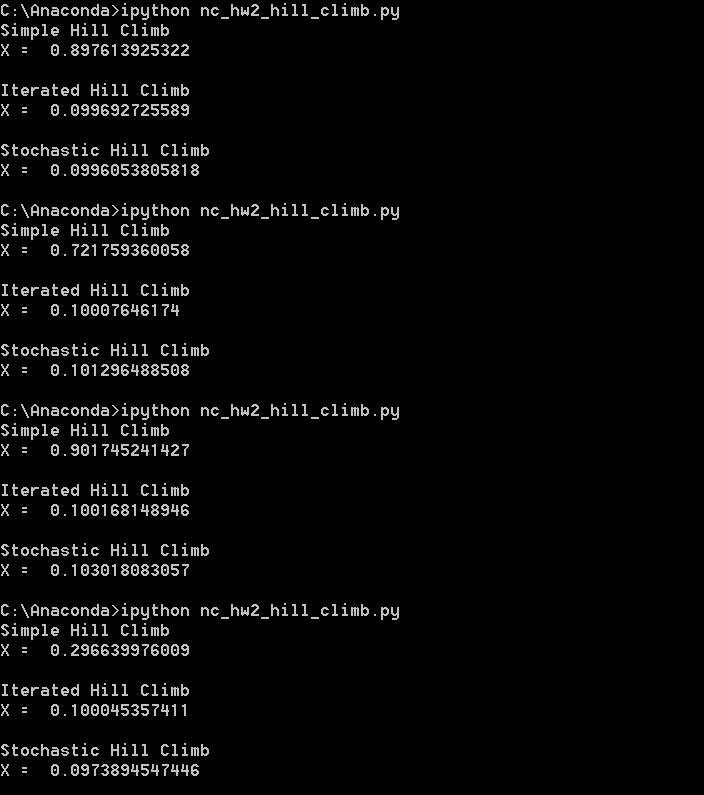
\includegraphics[width=0.75\textwidth]{HillClimb.PNG}
\end{center}
\caption{Sample Hill Climb Algorithms Answers \label{hill_climb} }
\end{figure}


\newpage
\section{Problem 2}
\textbf{Implement and apply the hill-climbing, simulated annealing, and genetic algorithms to maximize function $g(x)$ used in the previous exercise assuming a bitstring representation.} \newline \\
\textbf{Tip: The pertubation to be introduced in the candidate solutions for the hill-climbing and simulated annealing algorithms may be implemented similarly to the point mutation in genetic algorithms. Note that in this case, no concern is required about the domain of x, because the binary representation already accounts for it.} \newline \\
\textbf{Discuss the performance of the algorithms and asses their sensitivity in relation to the input parameters.}

\subsection{Summary}
Expanding on the evaluations in the previous problem we add a simple genetic algorithm to the mix. As mentioned, many of the solutions above can find themselves caught in a local extrema for many optimization problems. The genetic algorithm (granted a large enough initial population) avoids this problem by sampling a larger area of the search space.

\subsection{Implementation}
The code can be found in Listing~\ref{Problem2EA.py}.

\subsubsection{Encoding}
For the gene encoding, we used an unsigned 16 bit integer. This gave us an easy way to store 16 bits. Since we know the domain of the problem is restricted to $[0, 1]$ decoding the genotype into a phenotype was done by dividing the integer value of the bit string by the maximum value of a 16 bit integer (65535). Because the values are stored as integers, we can use numpy's random\_integers function to initialize the population.

\subsubsection{Crossover \& Mutation}
Crossover and mutation were handled by binary operations. Binary masks were stored in lists for each operator and a random index into those lists was generated to pick the mask used.

For mutation the individual was XOR'd with the mask to flip the proper bit. For crossover one parent was AND'd with the chosen mask and the other was AND'd with that masks negation. These values were then OR'd together to make the child individual.

\subsubsection{Selection}
Since our fitness values were simply the y values of the function and maximizing the function was the goal, a simple roulette selection method was chosen.

To avoid having to mess with the list of fitness values, an unused index list is created, and this is what the indexes are chosen from. Iterating through the unused list we add the value at that list to a variable until it is greater than or equal to a random value between 0 and the summation.

Between choosing each index the value at the chosen index is subtracted from the sum to avoid having to sum the unused values again. Unfortunately, since this uses floating point calculations it occasionally didn't reach the sum before the algorithm ran out of indexes. We fixed this problem by defaulting to the last index if the sum hasn't been reached by that point.

\subsection{Analysis}
Through multiple runs with different parameters, it was found that a genetic algorithm could solve this problem consistently with an initial population as low as 10 individuals in 250 iterations. The fastest consistent solution came from runs with around 100 individuals and 100 iterations. If more iterations were run it was able to get more precise, giving an answer of .0999923704891 for a max of .999999956813. Taking into account that the encoding isn't perfect this probably means we have the global max at .1 with a value of 1.


\newpage
\section{Problem 7}
\textbf{Determine, using genetic programming (GP), the computer program (S-expression) that produces exactly the outputs presented in Table 3.3 for each value of x. The following hypotheses are given:}
\begin{itemize}
\item \textbf{Use only functions with two arguments (binary trees).}
\item \textbf{Largest depth allowed for each tree: 4}
\item \textbf{Function set: F = {+, *}}
\item \textbf{Terminal set: T = {0, 1, 2, 3, 4, 5, x}}
\end{itemize}
\centerline{\begin{tabular}{ c c }
\hline
x & Program output \\
\hline
-10 & 153 \\
\hline
-9 & 120 \\
\hline
-8 & 91 \\
\hline
-7 & 66 \\
\hline
-6 & 45 \\
\hline
-5 & 28 \\
\hline
-4 & 15 \\
\hline
-3 & 6 \\
\hline
-2 & 1 \\
\hline
-1 & 0 \\
\hline
0 & 3 \\
\hline
1 & 10 \\
\hline
2 & 21 \\
\hline
3 & 36 \\
\hline
4 & 55 \\
\hline
5 & 78 \\
\hline
6 & 105 \\
\hline
7 & 136 \\
\hline
8 & 171 \\
\hline
9 & 210 \\
\hline
10 & 253 \\
\hline
\end{tabular}}

\subsubsection{Summary}
For this problem we originally intended to use BNF encoding and the related crossover and mutation operators with it. We were not able to get BNF encoding to work well as we were unsure of how to validate a string of integers as being a valid string. We then moved to an adapted simple genetic algorithm that worked on a prefix format equation. From that point validating the string, and that the resulting tree was limited to a depth of four was much easier.

\subsubsection{Encoding}
As stated above the encoding is as a prefix formatted equation. This format is easy to do crossover with (when we set the format of the equation in stone), but mutation has to check for two different cases of mutation. One for operators and one for terminals. The operators and terminals are given from the problem and explicitly stated below. \\
\centerline{
\begin{tabular}{| c | c |}
\hline
Operators & Terminals \\
\hline
	& 0 \\
	& 1 \\
+	& 2 \\ 
*	& 3 \\
	& 4 \\
	& 5 \\
	& x \\
\hline
\end{tabular}} \\

To simplify the encoding process, we started with a default encoding and then used the mutation operator to randomize the initial population. The default encoding can be seen below. \\

\centerline{+ + + 0 0 + 0 0 + + 0 0 + 0 0} \hfill \\

This evaluates to the following tree:

\centerline{
\begin{minipage}{.5\linewidth}
\centerline{+ } \hfill \\
\centerline{\hfill + \hfill + \hfill } \hfill \\
\centerline{\hfill + \hfill + \hfill + \hfill + \hfill } \hfill \\
\centerline{\hfill 0 \hfill 0 \hfill 0 \hfill 0 \hfill  0 \hfill 0 \hfill 0 \hfill 0 \hfill} \hfill \\
\end{minipage}}

As you can see, this is not a particularly useful individual, so we copy it and randomize it through mutation to sample the search space.

\subsubsection{Crossover \& Mutation}
Crossover was even simpler in this problem than in the previous. Our prefix equation was stored as a list of strings, so we split the list at a random crossover point and split and recombined the mother and father into a child.

Mutation was more complicated in this problem but only marginally so. The complication was that there are two parts to the individuals using our encoding. There were the operators and the terminals. Since the locations of these are fixed, we stored the locations of each in a separate list, and if our randomly selected mutation index is in the operator index list we replace the value with a random operator. If the mutation index is in the terminals index list we replace the value with a random terminal.

\subsubsection{Selection}
The roulette selection operator from the previous problem was reused. To make it work properly, the evaluation function had to be modified significantly. Our first instinct was to add up the difference between the expected and found values. This was easy to implement so we went with it, but this evaluation function does the exact opposite of what we want. It creates high values for less fit individuals. We solved this by finding the maximum value and then replacing every individual's fitness with $(max - fitness) / max$. This normalized the values between 0 and 1 and made them be the proper fitness relative to each other.

\subsubsection{Analysis}
The hardest part of this problem was to choose a good representation for the individuals. The prefix notation worked well and forcing a format that expanded to a full depth four tree simplified a lot of the process.

When using a population of 250 and up to 1000 iterations (up to because we can short circuit the process if we find a perfect solution) we calculated a \%100 match 100 times out of 100. The full list of these can be found in Appendix~\ref{results.out}.

Because we didn't want to fully analyze 100 different prefix notation equations, we randomly picked 10 to evaluate. These are listed below.



\chapter{Artificial Neural Networks - Text Chapter 4}

\section{Problem 17}

\textbf{Apply the MLP network trained with the backpropagation learning algorithm to solve the character recognition task of Section 4.4.2.} \newline \\
\textbf{Determine a suitable network architecture and then test the resultant network sensitivity to noise the the test data. Test different noise levels, from 5\% to 50\%}



% !TEX root = BioInspired.tex

\chapter{Swarms - Text Chapter 5}

\section{ Problem 1 }
\textbf{Write a pseudocode for the simple ACO (S-ACO) algorithm considering pheromone evaportation, implement it computationally, and apply it to solve the TSP instance presented in Section 3.10.4. Discuss the results obtained.} \newline \\
\textbf{Remove the pheromone evaportation term (Equation ~\ref{eqn5.3}), apply the alogorithm to the same problem, and discuss the results obtained.}

\begin{equation} \label{eqn5.3}
\tau_{ij}(t) \leftarrow ( 1-\rho ) \tau_{ij}(t) + \Delta \tau
\end{equation}

% Problem 1 Discussion

\subsection{Summary}
The Traveling Salesman Problem is a popular problem in the field of computer science. The idea is there is a list of cities a salesman wants to visit, for the cheapest cost. In this problem, ant colony optomization is used to a find a low-cost solution.

\subsection{Implementation}
Code for this may be found in Listing~\ref{tsp_aco.cpp}.

The pseudocode for the simple ant colony optomization is presented in subsection ~\ref{acoPseudo}. This pseudocode has gone through a few revisions as code was written and moments of ``That's not going to work.'' occured. 

First, cities and their locations are read from a file and used to create a 2D array of edges with associated distances, pheromones, and visibilties. Next, a solution for each ant is built. A node is randomly selected for the starting point, a probability list (for moving to the next unvisited node) is constructed using Equation ~\ref{eqn5.5}, a random value is generated and checked against the probability list to see which node is next moved to. The selected node is then removed from the available nodes list, added to the visited list, and pheromone added to the edge. This repeats for each node until all nodes have been traversed.

\begin{equation} \label{eqn5.5}
p_{ij}^{k}(t) = 
	\begin{cases}
	\frac{ [\tau_{ij}(t)]^\alpha [\eta_{ij}]^\beta} {\Sigma_{l \in J_i^k}[\tau_{il}(t)]^\alpha[\eta_{il}]^\beta } & \text{if} j \in J_i^k \\
	0 	& \text{otherwise} \\
	\end{cases}
\end{equation}

Once the visited list for each ant has been built, the fitness of each path will be evaluated. To determine the fitness, it will simply be the total length of all edges. The most fit path will be the shortest path. Then, Equation ~\ref{eqn5.2} is applied to all edges to simulate the `evaporation' of pheromones. 

\begin{equation} \label{eqn5.2}
\tau_{ij}(t) \leftarrow \tau_i(t) + \Delta \tau
\end{equation}

\subsection{Analysis}
There's a bug in the bug code. A struct to contain edge information such as start node, end node, pheromone level, distance and visibilty was created. Then a 2D array of those structs was created to hold all possible edges. The 2D array is filled such that no edge is repeatedly stored, so half of the array is filled. Pheromone is intialized to one for all edges. 

During debugging of the move function, when accessing the pheromone information, occasionally the pheromone data would be 0 instead of 1. This could be an indexing issue, but on 3 hours of sleep, and checking the logic against several people, Stephanie can't figure out what's wrong. One would think that she would have learned from McGough's robotics class, his homeworks should really be started more than one week before it's due (even if that week is spring break).

% S-ACO pseudocode
\subsection{ S-ACO Pseudocode } \label{acoPseudo}
\begin{lstlisting}
SACO( max_it, ants, edges )
{
	t = 0
	while ( t < max_it )
	{
		// for each ant
		// place ant on randomly selected node
		
		for( i = 0; ants; i++)
		{
			// calculate probability of moving to each untraveled node
			// use probabalistic move rule to determine next node
			// mark new node as traveled
			// add node to traveled path
		}
		
		// evaluate cost of each solution
		if ( solution < best )
			best = solution

		//update pheromone trails
		t++
	}
}
\end{lstlisting}


\section{ Problem 8 }
\textbf{Apply the PS algorithm described in Section 5.4.1 to the maximization problem of Example 3.3.3. Compare the relative performance of the PS algorithm with that obtained using a standard genetic algorithm.} \newline 

\subsection{Summary}
Expanding upon the evolutionary algorithms to solve the maximization problem of Example 3.3.3 in the book, a particle swarm approach is implemented and compared against the evoluationary algorithms.

\subsection{Implementation}
Random points along the x-axis between zero and one are initialized as the population. Each individual is then assigned a random initial velocity between zero and one. Next, each individual's fitness is then evaluated and the best fit individual is tracked. Then a loop is entered for a specified number of time steps. During each time step, each individual's velocity is slightly perturbed, the fitness re-evaluatated, and new best fit positions are tracked. The code can be found in Listing~\ref{pso.cpp}.

\subsection{Analysis}
The trials for this implementation were run with varing a population size from ten to twenty and time steps from ten to 200. Consistent answers were obtained with a population of fifteen and ten steps. When the population was dropped to ten, the correct answer would be calculated approximently 50\% of the time. Figure ~\ref{psoRun} shows some sample runs. The genetic algorithm consistently found correct solutions with a population as low as 10 and 100 steps. So, computationally, the particle swarm approach is faster than the genetic algorithm for this particular problem. 

\begin{figure}[tbh]
\begin{center}
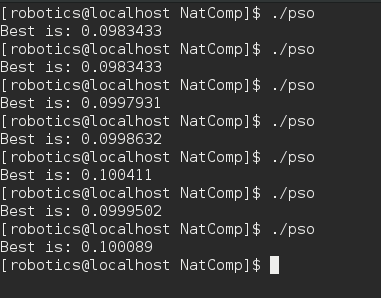
\includegraphics[width=0.5\textwidth]{psoRUN.png}
\end{center}
\caption{ Sample Particle Swarm Answers } \label{psoRun}
\end{figure}
% !TEX root = BioInspired.tex

\chapter{Immunocomputing - Text Chapter 6}

\section{Problem 1}
\textbf{Use a bone marrow algorithm to define genes for gene libraries to be used to generate the initial population of a genetic algorithm to solve the TSP problem presented in Chapter 3 and Chapter 5 (Figure 6.24). Assume the following structure for the gene libraries:}

\textbf{Gene length $L_g = 4$, number of libraries $n = 8$, and library length (number of genes in each library) $L_l = 4$. As one gene for each library will be selected, the total chromosome length is $L = Lg \times n = 4 \times 8 = 32$, that corresponds to the number of cities in a tour.}

\textbf{Each gene will be defined as a sequence of four cities known to be part of an optimal route. Since many of the chromosomes produced will contain repeated values, a repair function must be created.}

\textbf{Implement this bone marrow model to define an initial population of chromosomes to be used in an evolutionary algorithm to solve the TSP problem illustrated. Compare the performance of the algorithm with this type of initialization procedure and with the random initialization used in Project 1, Section 3.10.4}

\subsection{Summary}
Since we did not do Project 1 for this homework assignment, we won't be comparing the performance of the populations. This algorithm is pretty simple, so we packaged it into a reusable class for future work. The code can be found in Listing~\ref{BoneMarrow.py}.

\subsection{Implementation}
As stated above, we packaged the process into a generic class to allow it to be used for various problems.

\subsubsection{Libraries}
We decided to let there be two methods of adding a library. You can add a complete library, or create a library with a gene generator function. In some initial thoughts, a mutator function could also be passed in, but this was out of the scope of the function and not necessary for the problem.

\subsubsection{Chromosomes}
With our class you can create single or sets of chromosomes. The chromosomes are run through a repair function that is passed into the constructor of the class before being returned or added to the return list. The method of making the chromosomes is pretty straight forward. Start with a random element from the first library and add random genes from the rest of the libraries in the order added until the chromosome is complete.

\subsection{Analysis}
This seems to be a quick way to generate more complex encodings than using a purely random method. It would have been a nice addition to Chapter~3~Problem~7, as the prefix notation was made of very specific parts, but they were different from each other and had to go in order. It may be used in that problem for future analysis

In our testing two different generators were used, one with random strings for genes, and one with a subset of the optimal path (seen in Figure~6.24 in the text). Running the python file generates and prints both of these sets to the screen.
% !TEX root = BioInspired.tex

\chapter{Latex}
Big ole grab bag of latex sample code ....


\section{Some \LaTeX\ }

See Figure~\ref{systemdiagram}.  This is a floating
figure environment.  \LaTeX\ will try to put it close to where it was
typeset but will not allow the figure to be split if moving it can not
happen.  Figures, tables, algorithms and many other floating
environments are automatically numbered and placed in the appropriate
type of table of contents.  You can move these and the numbers will
update correctly.

\begin{figure}[tbh]
\begin{center}
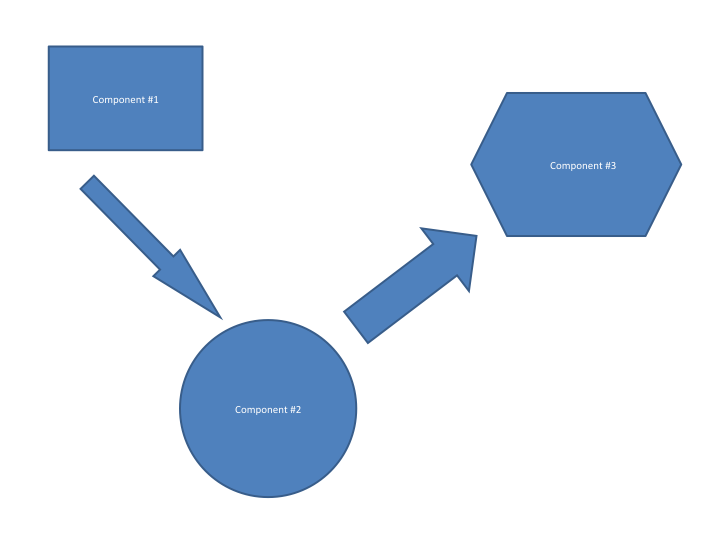
\includegraphics[width=0.75\textwidth]{./diagram}
\end{center}
\caption{A sample figure .... System Diagram \label{systemdiagram}}
\end{figure}




See Table~\ref{somenumbers}.  This is a floating table environment.
\LaTeX\ will try to put it close to where it was typeset but will not
allow the table to be split.

\begin{table}[tbh]
\caption{A sample Table ... some numbers. \label{somenumbers}}
\begin{center}
\begin{tabular}{|r|l|}
  \hline
  7C0 & hexadecimal \\
  3700 & octal \\ \cline{2-2}
  11111000000 & binary \\
  \hline \hline
  1984 & decimal \\
  \hline
\end{tabular}
\end{center}
\end{table}

Sample bullet list environment:
\begin{itemize}
\item According to the all knowing wikipedia, C is an all purpose imperative programming language.   
\item Developed between 1969 and 1973 by Dennis Ritchie.  [With help from Ken Thompson.]
\item One of the most influential computer languages.
\end{itemize}

Sample numbered list:
 \begin{enumerate}
 \item Predictor:  Small step in direction $\lambda \in {\cal N}(J_G(x))$:
\item Corrector:  $y^{k+1} = y^k + (J_G(y^k))^{-1}G(y^k,\lambda)$
\end{enumerate}

\section{Section\#1 }

Example Section.

\subsection{Subsection \#1}

Example subsection.

\subsubsection{Subsubsection \#1}

Because I can.   [But I did not assign a color to the font.]


\begin{equation}
\displaystyle\frac{\partial u}{\partial t} = k \left( \frac{\partial^2 u}{\partial x^2} +  \frac{\partial^2 u}{\partial y^2} \right)
\end{equation}

\subsection{Code Details}
Here is an example code listing:
\begin{lstlisting}
#include <stdio.h>
#define N 10
/* Block
 * comment */
 
int main()
{
    int i;
 
    // Line comment.
    puts("Hello world!");
 
    for (i = 0; i < N; i++)
    {
        puts("LaTeX is also great for programmers!");
    }
 
    return 0;
}
\end{lstlisting}
This code listing is not floating or automatically numbered.  If you want auto-numbering, but it in the algorithm environment (not algorithmic however) shown above.


Sample algorithm:  Algorithm~\ref{alg1}.  This algorithm environment is automatically placed - meaning it floats.   You don't have to worry about placement or numbering.  

\begin{algorithm} [tbh]                     % enter the algorithm environment
\caption{Calculate $y = x^n$}          % give the algorithm a caption
\label{alg1}                           % and a label for \ref{} commands later in the document
\begin{algorithmic}                    % enter the algorithmic environment
    \REQUIRE $n \geq 0 \vee x \neq 0$
    \ENSURE $y = x^n$
    \STATE $y \Leftarrow 1$
    \IF{$n < 0$}
        \STATE $X \Leftarrow 1 / x$
        \STATE $N \Leftarrow -n$
    \ELSE
        \STATE $X \Leftarrow x$
        \STATE $N \Leftarrow n$
    \ENDIF
    \WHILE{$N \neq 0$}
        \IF{$N$ is even}
            \STATE $X \Leftarrow X \times X$
            \STATE $N \Leftarrow N / 2$
        \ELSE[$N$ is odd]
            \STATE $y \Leftarrow y \times X$
            \STATE $N \Leftarrow N - 1$
        \ENDIF
    \ENDWHILE
\end{algorithmic}
\end{algorithm}
Citations look like~\cite{Choset:2005:PRM, arkin2009governing, lavalle2006}  and~\cite{wiki:asimo,lumelsky:1987, nolfi2000evolutionary}.  These are done automatically.  Just fill in the database {\tt designrefs.bib} using the same field structure as the other entries.  Then pdflatex the document, bibtex the document and pdflatex twice again.  The first pdflatex creates requests for bibliography entries.
The bibtex extracts and formats the requested entries.  The next pdflatex puts them in order and assigns labels.  The final pdflatex replaces references in the text with the assigned labels.
The bibliography is automatically constructed.  

\section{Section \#2}

An example of a minipage environment (gets side by side content - like two column mode).  Also there is an example of a flow chart using tikz.  
\noindent
Flowcharts\\[3mm]
\tikzstyle{startstop} = [rectangle, rounded corners, minimum width=3cm, minimum height=1cm,text centered, draw=black, fill=red!30]\tikzstyle{io} = [trapezium, trapezium left angle=70, trapezium right angle=110, minimum width=3cm, minimum height=1cm, text centered, draw=black, fill=blue!30]
\tikzstyle{process} = [rectangle, minimum width=3cm, minimum height=1cm, text centered, draw=black, fill=orange!30]
\tikzstyle{decision} = [diamond, minimum width=3cm, minimum height=1cm, text centered, draw=black, fill=green!30]
\tikzstyle{arrow} = [thick,->,>=stealth]
\begin{minipage}{0.45\textwidth}
\begin{tikzpicture}[node distance=2cm]
\node (start) [startstop] {Start};
\node (in1) [io, below of=start] {Input};
\node (pro1) [process, below of=in1] {Process 1};
\node (dec1) [decision, below of=pro1] {Decision 1};
\end{tikzpicture}\\
\begin{picture}(0,0)
\put(0,0){Flow:   \vector(1,0){40}}
\end{picture}
\end{minipage}
\begin{minipage}{0.45\textwidth}
\begin{tikzpicture}[node distance=2cm]
\node (start) [startstop] {Start};
\node (in1) [io, below of=start] {Input};
\node (pro1) [process, below of=in1] {Process 1};
\node (dec1) [decision, below of=pro1, yshift=-0.5cm] {Decision 1};
\node (pro2a) [process, below of=dec1, yshift=-0.5cm] {Process 2a};
\node (pro2b) [process, right of=dec1, xshift=2cm] {Process 2b};
\node (out1) [io, below of=pro2a] {Output};
\node (stop) [startstop, below of=out1] {Stop};
\draw [arrow] (start) -- (in1);
\draw [arrow] (in1) -- (pro1);
\draw [arrow] (pro1) -- (dec1);
\draw [arrow] (dec1) -- (pro2a);
\draw [arrow] (dec1) -- (pro2b);
\draw [arrow] (dec1) -- node[anchor=east] {yes} (pro2a);
\draw [arrow] (dec1) -- node[anchor=south] {no} (pro2b);
\draw [arrow] (pro2b) |- (pro1);
\draw [arrow] (pro2a) -- (out1);
\draw [arrow] (out1) -- (stop);
\end{tikzpicture}
\end{minipage}



More in the sample document at the end.


%%%  Done with chapters
% Bib stuff

\bibliographystyle{plain}
\bibliography{refs.bib}
\addcontentsline{toc}{chapter}{Bibliography}



% In our style file, appendices are numbered with capital letters
\appendix

\chapter{Supporting Materials}

This document will contain several appendices used as a way to separate out major 
component details, logic details, or tables of information.  Use of this structure 
will help keep the document clean, readable, and organized. 



\chapter{Code}
\includecode{Problem2EA.py}

\newpage
\includecode{pso.cpp}

\newpage
\includecode{tsp_aco.cpp}

\newpage
\includecode{nc_hw2_hill_climb.py}

\newpage
\includecode{BoneMarrow.py}


% chapters in backmatter don't have numbers, but they appear in the
% table of contents, and are numbered BM-X where X is the page number
% relative to where the backmatter begins.
\backmatter


%%  The author of LaTeX provided all of us with a sample document.  Here it is ...
\chapter{\LaTeX\ Example}
% !TEX root = BioInspired.tex


\LaTeX\xspace sample file:  

\section{Introduction}
This is a sample input file.  Comparing it with the output it
generates can show you how to produce a simple document of
your own.

\section{Ordinary Text}  % Produces section heading.  Lower-level
                                    % sections are begun with similar 
                                    % \subsection and \subsubsection commands.

The ends  of words and sentences are marked 
  by   spaces. It  doesn't matter how many 
spaces    you type; one is as good as 100.  The
end of   a line counts as a space.

One   or more   blank lines denote the  end 
of  a paragraph.  

Since any number of consecutive spaces are treated like a single
one, the formatting of the input file makes no difference to
      \TeX,         % The \TeX command generates the TeX logo.
but it makes a difference to you.  
When you use
      \LaTeX,       % The \LaTeX command generates the LaTeX logo.
making your input file as easy to read as possible
will be a great help as you write your document and when you
change it.  This sample file shows how you can add comments to
your own input file.

Because printing is different from typewriting, there are a 
number of things that you have to do differently when preparing 
an input file than if you were just typing the document directly.  
Quotation marks like 
       ``this'' 
have to be handled specially, as do quotes within quotes: 
       ``\,`this'                  % \, separates the double and single quote.
        is what I just 
        wrote, not  `that'\,''.  

Dashes come in three sizes: an 
       intra-word 
dash, a medium dash for number ranges like 
       1--2, 
and a punctuation 
       dash---like 
this.

A sentence-ending space should be larger than the space between words
within a sentence.  You sometimes have to type special commands in
conjunction with punctuation characters to get this right, as in the
following sentence.
       Gnats, gnus, etc.\    % `\ ' makes an inter-word space.
       all begin with G\@.   % \@ marks end-of-sentence punctuation.
You should check the spaces after periods when reading your output to
make sure you haven't forgotten any special cases.
Generating an ellipsis 
       \ldots\    % `\ ' needed because TeX ignores spaces after 
                  % command names like \ldots made from \ + letters.
                  %
                  % Note how a `%' character causes TeX to ignore the 
                  % end of the input line, so these blank lines do not
                  % start a new paragraph.
with the right spacing around the periods 
requires a special  command.  

\TeX\ interprets some common characters as commands, so you must type
special commands to generate them.  These characters include the
following: 
       \$ \& \% \# \{ and \}.

In printing, text is emphasized by using an
       {\em italic\/}  % The \/ command produces the tiny extra space that
                       % should be added between a slanted and a following
                       % unslanted letter.
type style.  

\begin{em}
   A long segment of text can also be emphasized in this way.  Text within
   such a segment given additional emphasis 
          with\/ {\em Roman} 
   type.  Italic type loses its ability to emphasize and become simply
   distracting when used excessively.  
\end{em}

It is sometimes necessary to prevent \TeX\ from breaking a line where
it might otherwise do so.  This may be at a space, as between the
``Mr.'' and ``Jones'' in
       ``Mr.~Jones'',        % ~ produces an unbreakable interword space.
or within a word---especially when the word is a symbol like
       \mbox{\em itemnum\/} 
that makes little sense when hyphenated across 
       lines.

Footnotes\footnote{This is an example of a footnote.}
pose no problem.

\TeX\ is good at typesetting mathematical formulas like
       \( x-3y = 7 \) 
or
       \( a_{1} > x^{2n} / y^{2n} > x' \).
Remember that a letter like
       $x$        % $ ... $  and  \( ... \)  are equivalent
is a formula when it denotes a mathematical symbol, and should
be treated as one.

\section{Displayed Text}

Text is displayed by indenting it from the left margin.
Quotations are commonly displayed.  There are short quotations
\begin{quote}
   This is a short a quotation.  It consists of a 
   single paragraph of text.  There is no paragraph
   indentation.
\end{quote}
and longer ones.
\begin{quotation}
   This is a longer quotation.  It consists of two paragraphs
   of text.  The beginning of each paragraph is indicated
   by an extra indentation.

   This is the second paragraph of the quotation.  It is just
   as dull as the first paragraph.
\end{quotation}
Another frequently-displayed structure is a list.
The following is an example of an {\em itemized} list.
\begin{itemize}
   \item  This is the first item of an itemized list.  Each item 
          in the list is marked with a ``tick''.  The document
          style determines what kind of tick mark is used.

   \item  This is the second item of the list.  It contains another
          list nested inside it.  The inner list is an {\em enumerated}
          list.
          \begin{enumerate}
              \item This is the first item of an enumerated list that
                    is nested within the itemized list.

              \item This is the second item of the inner list.  \LaTeX\
                    allows you to nest lists deeper than you really should.
          \end{enumerate}
          This is the rest of the second item of the outer list.  It
          is no more interesting than any other part of the item.
   \item  This is the third item of the list.
\end{itemize}
You can even display poetry.
\begin{verse}
   There is an environment for verse \\    % The \\ command separates lines
   Whose features some poets will curse.   % within a stanza.

                           % One or more blank lines separate stanzas.

   For instead of making\\
   Them do {\em all\/} line breaking, \\
   It allows them to put too many words on a line when they'd 
   rather be forced to be terse.
\end{verse}

Mathematical formulas may also be displayed.  A displayed formula is
one-line long; multi-line formulas require special formatting
instructions.
   \[  x' + y^{2} = z_{i}^{2}\]
Don't start a paragraph with a displayed equation, nor make
one a paragraph by itself.

\section{Build process}

To build \LaTeX\ documents you need the latex program.  It is free and available on all operating systems.   Download and install.  Many of us use the TexLive distribution and are very happy with it.    You can use a editor and command line or use an IDE.  To build this document via command line:

\begin{verbatim}
alta>  pdflatex SystemTemplate
\end{verbatim}
If you change the bib entries, then you need to update the bib files:
\begin{verbatim}
alta>  pdflatex SystemTemplate
alta>  bibtex SystemTemplate
alta>  pdflatex SystemTemplate
alta>  pdflatex SystemTemplate
\end{verbatim}

The template files provided also contain a Makefile, which will
make things much easier.  

\section*{Acknowledgment}
Thanks to Leslie Lamport.  






\end{document}
